\appendix
\label{sec:appendix}

\section{Comparison with other topic model}

\par In this section we apply other topic model, Latent Dirichlet Allocation \cite{blei2003latent} (LDA), to our corpus and compare its results to the shown in this paper. Due to the increasingly use of LDA, we think that a few words about the performance of LDA in our work is necessary. 

\par Naturally the topics found with LDA may not coincide with the NMF ones.
However, one expects that the corpus under studying should be in some manner robust to the election of the topic model.
On the other hand, as was discussed in \cite{o2015analysis}, NMF can be a more suitable topic modeling method in certain domains, in the way that it produces more coherent topics, while LDA tends to return higher levels of generality and redundancy. Topic coherence is defined as the semantic interpretability of the terms used to describe a particular topic, although the coherence of a topic may depend on the end user's expectations.

\par We define a simple coherence measure defined in equation \ref{eq:topic_coherence}, where $d_{ij}$ is the number of documents where the term $i$ and term $j$ appear simultaneously, and $d_{x}$ is the number of documents where appears the term $x$. The summation is over the $N$ top terms of the topic.
It's important to note that if two terms have no co-occurrences, the contribution to the summation is zero, and if these ones appear only together the contribution is one.
A topic with higher coherence is a topic where the terms that define it co-occurrence frequently.

\begin{equation}
TC = \sum_{i < j}^N \frac{2d_{ij}}{d_i + d_j}
\label{eq:topic_coherence} 
\end{equation}

\par We perform a decomposition into 10 topics using LDA with the python module \emph{gensim} \cite{rehurek_lrec}, which allow us to modify the number of times the corpus is read, improving the coherence of the topics.
Unlike to what we see with NMF, the LDA's performance depends strongly on the initial condition of the algorithm. After 10 iterations, we chose the one with highest mean topic coherence, and compared this with the NMF results.

\par In figure \ref{fig:temporal_profiles_nmf_lda} we show the temporal profiles of topics \emph{Elections} and \emph{Missing Person} for both NMF and LDA. The association between topic models was simply made by looking at the topics which share common keywords.
As can be seen from the figure and the table \ref{table:correlation_nmf_lda}, those LDA topics which can be linked to NMF ones or to a combination of these, show a temporal profile highly correlated. 

\par Nevertheless, LDA returns other topics which can not be directly associated, some of them composed of very general words. 
By keeping only those topics which can be associated with NMF and re-defining the Media Agenda over this topic space with reduced dimension, we observed similar results by both methods.  
The same procedure is proposed in absence of an alternative topic model to which make the comparison: Keep only those topics easily interpretable and define the Agendas over this reduced space.
 
\begin{figure}
\centering
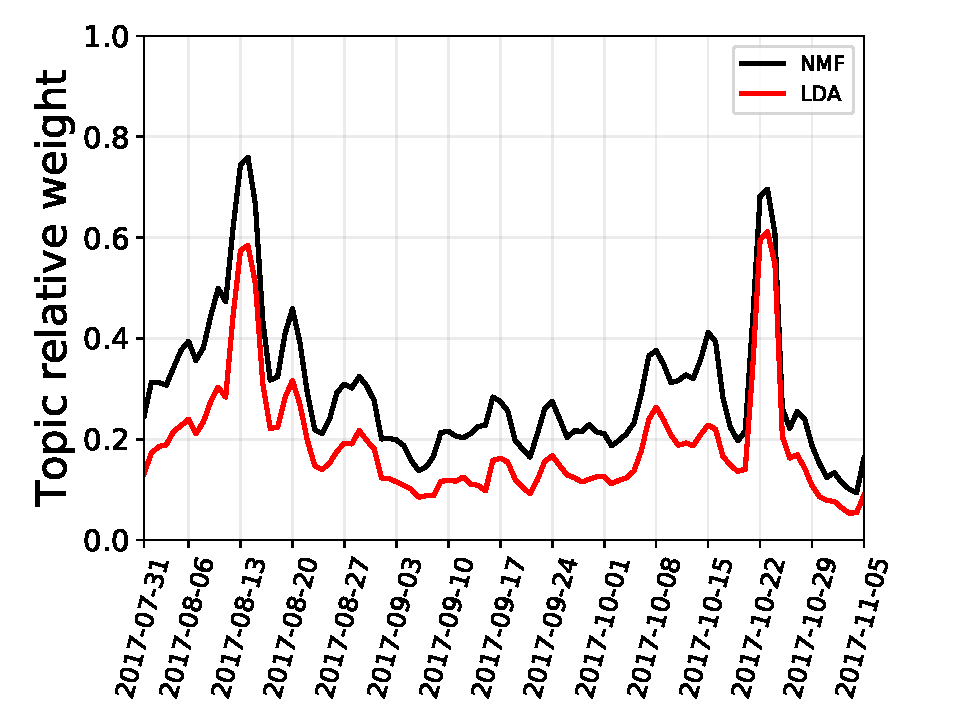
\includegraphics[scale = 0.4]{images/FigA2.pdf}
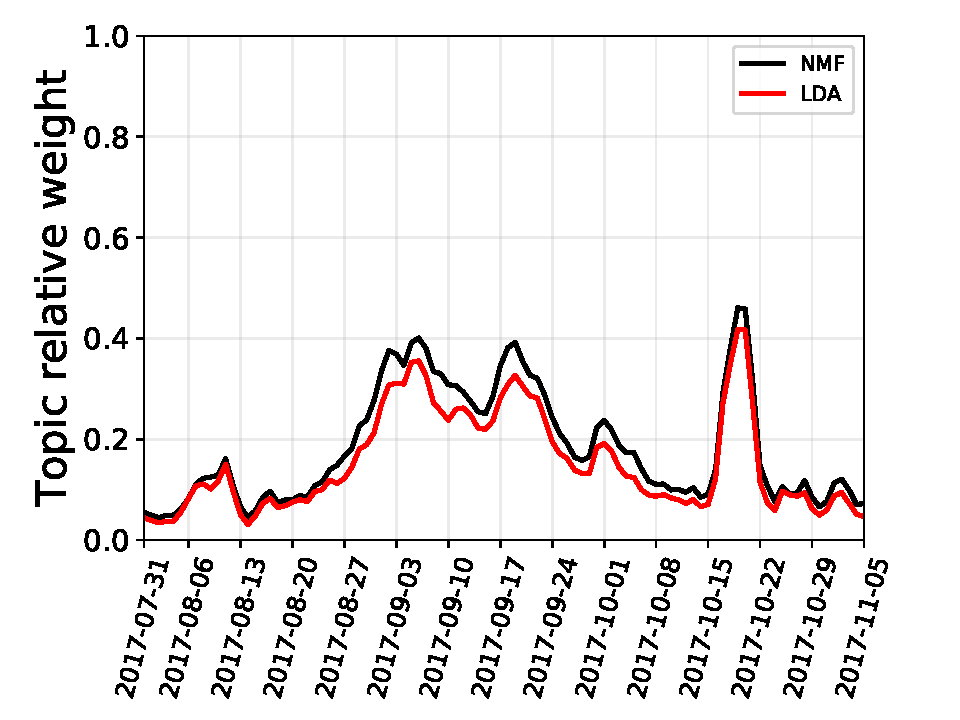
\includegraphics[scale = 0.4]{images/FigA1.pdf}
\caption{Temporal profiles of topics \emph{Elections} (left) and \emph{Missing Person} (right) for both LDA and NMF. All the topics found by applying NMF have a highly correlated counterpart in LDA.} 
\label{fig:temporal_profiles_nmf_lda}
\end{figure}

\begin{table}[h]
\centering
\resizebox{\textwidth}{!}{\begin{tabular}{llc}
\toprule
& Correlation between NMF and LDA \\
\midrule
Elections & \textbf{0.98} \\
Missing person & \textbf{0.99} \\
Former Planning minister + Former Vice-President & \textbf{0.89} \\
Current President & \textbf{0.94} \\
Social leader & \textbf{0.94} \\
Prosecutor's death & \textbf{0.83} \\
\bottomrule
\end{tabular}}
\caption{Correlation between the temporal profiles of the topics found in NMF and associated topics in LDA.}
\label{table:correlation_nmf_lda}
\end{table}
 


